\documentclass[12pt]{beamer}
\usetheme{Warsaw}
\usepackage[utf8]{inputenc}
\usepackage[spanish]{babel}
\usepackage{amsmath}
\usepackage{amsfonts}
\usepackage{amssymb}
\usepackage{graphicx}
\usepackage{color}
\definecolor{softgray}{rgb}{0.8,0.8,0.8}
\usepackage{listings} %Para codigo
\author{Daniel Bolaños Martínez, José María Borrás Serrano, Santiago De Diego De Diego, Fernando De la Hoz Moreno}
\title{Práctica 2: Algoritmos Divide y Vencerás}
\setbeamercovered{transparent} 
\setbeamertemplate{navigation symbols}{} 
%\logo{} 
\institute{ETSIIT} 
\date{} 

%\subject{} 
\begin{document}

\begin{frame}
\titlepage
\end{frame}

\begin{frame}{Introducción}

\end{frame}

\begin{frame}[fragile]{Código Divide y Vencerás}
	\lstset{language=C++, breaklines=true, backgroundcolor=\color{softgray},keywordstyle=\color{blue},stringstyle=\color{orange},basicstyle=\footnotesize}
	\begin{lstlisting}
	
	\end{lstlisting}
\end{frame}

\begin{frame}[fragile]{Código secuencial}
	\lstset{language=C++, breaklines=true, extendedchars=true,backgroundcolor=\color{softgray}, keywordstyle=\color{blue},stringstyle=\color{orange},caption={Función unimodal DyV}, basicstyle=\tiny}
	\begin{lstlisting}
int unimodal(vector<int> v)
{
	bool fin=false;
	int maximo=v.size()-1;
	int indice=maximo/2;
	int minimo;
 
	while(!fin)
	{
        if(v.at(indice-1)<v.at(indice))
           if(v.at(indice+1)<v.at(indice))
			    fin=true;
		   else
		   {
				minimo=indice;
				indice=indice+((maximo-indice)/2);
			}
		else
		{
			maximo=indice;
			indice=minimo+((indice-minimo)/2);
		}
	}
	return indice;
}
	\end{lstlisting}
\end{frame}
\begin{frame}[fragile]
	\lstset{language=C++, breaklines=true, extendedchars=true, caption={Función main DyV},backgroundcolor=\color{softgray},keywordstyle=\color{blue},stringstyle=\color{orange},basicstyle=\tiny}
	\begin{lstlisting}
int main(int argc, char* argv[])
{
	vector<int> array;
  	int valor = -1;
	double suma=0;

	int v_size = atoi(argv[1]);
	array.resize(v_size);

	for(int i=0; i<100; ++i)
	{
		int p = 1 + rand() % (v_size-2);
  		array.at(p) = v_size-1;
  		for (int i=0; i<p; i++)
  			array.at(i)=i;
  		for (int i=p+1; i<v_size; i++)
  			array.at(i)=v_size-1-i+p;

		clock_t tantes;
		clock_t tdespues;
		tantes=clock();
		valor = unimodal(array);
		tdespues=clock();
		suma += (double)(tdespues - tantes) / CLOCKS_PER_SEC;
	}
  	cout << v_size <<" "<< suma/100 << endl;
}
	\end{lstlisting}

\end{frame}

\begin{frame}[fragile]{Código secuencial}
	\lstset{language=C++, breaklines=true, extendedchars=true,backgroundcolor=\color{softgray}, keywordstyle=\color{blue},stringstyle=\color{orange},caption={Función unimodal Secuencial}, basicstyle=\footnotesize}
	\begin{lstlisting}
int unimodal_secuencial(vector<int> v)
{
	bool fin=false;
  	int indice=1;

  	while(!fin)
  	{
     	if(v.at(indice+1)<v.at(indice))
      		fin=true;
     	else
      		indice++;
  	}

  	return indice;
}
	\end{lstlisting}
\end{frame}

\begin{frame}[fragile]
	\lstset{language=C++, breaklines=true, extendedchars=true, caption={Función main Secuencial},backgroundcolor=\color{softgray},keywordstyle=\color{blue},stringstyle=\color{orange},basicstyle=\tiny}
	\begin{lstlisting}
int main(int argc, char* argv[])
{
	vector<int> array;
  	int valor = -1;
	double suma=0;

  	int v_size = atoi(argv[1]);
  	array.resize(v_size);

	for(int i=0; i<100; ++i)
	{
		int p = 1 + rand() % (v_size-2);
  		array.at(p) = v_size-1;
  		for (int i=0; i<p; i++)
  			array.at(i)=i;
  		for (int i=p+1; i<v_size; i++)
  			array.at(i)=v_size-1-i+p;

  		clock_t tantes;
  		clock_t tdespues;
  		tantes=clock();
  		valor = unimodal_secuencial(array);
  		tdespues=clock();
		suma += (double)(tdespues - tantes) / CLOCKS_PER_SEC;
	}
  	cout << v_size <<" "<< suma/100 << endl;
}
	\end{lstlisting}

\end{frame}

\begin{frame}{Eficiencia en el caso secuencial}

\begin{figure}[H] 
\centering
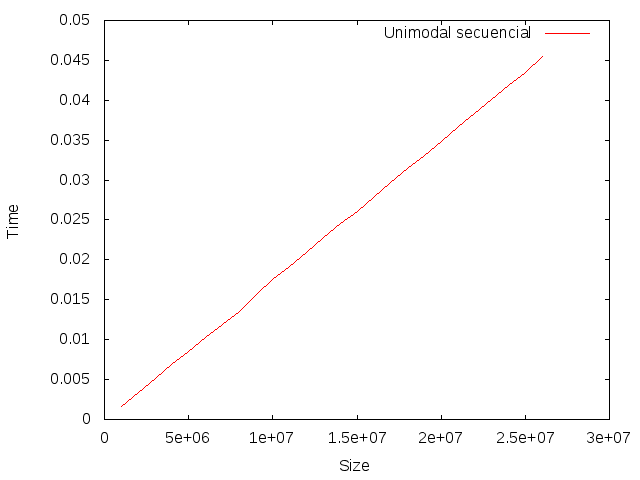
\includegraphics[angle=0,scale=0.5]{img/Eficiencia_sec.png} 
\end{figure}

\end{frame}

\begin{frame}{Eficiencia en el caso Divide y Vencerás}

\begin{figure}[H] 
\centering
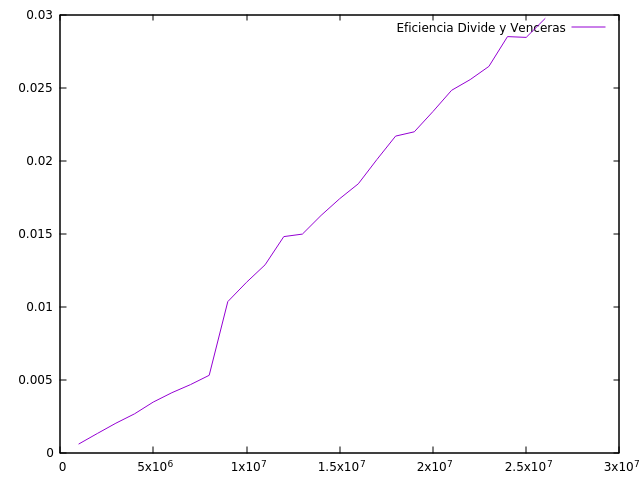
\includegraphics[angle=0,scale=0.5]{img/Eficiencia_dyv.png} 
\end{figure}

\end{frame}

\begin{frame}{Ajuste híbrido en el caso secuencial}

\begin{figure}[H] 
\centering
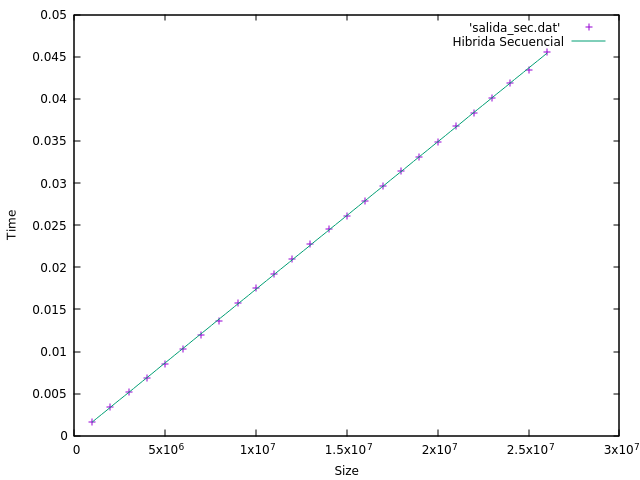
\includegraphics[angle=0,scale=0.5]{img/AjusteHibridoSec.png} 
\caption{Pie de imagen} 
\end{figure}

\end{frame}

\begin{frame}{Ajuste híbrido en el caso Divide y Vencerás}

\begin{figure}[H] 
\centering
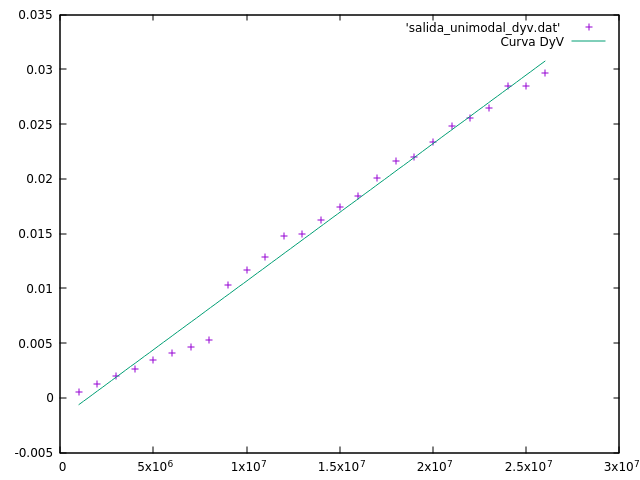
\includegraphics[angle=0,scale=0.5]{img/AjusteHibridoDyV.png} 
\caption{Pie de imagen} 
\end{figure}

\end{frame}

\begin{frame}{Conclusión}

\end{frame}

\end{document}
